\documentclass[italian,12pt,a4paper]{article}
\usepackage[utf8]{inputenc}
\usepackage[T1]{fontenc}
\usepackage{mathtools}
\usepackage{blkarray, bigstrut} %
\usepackage{babel}
\usepackage{graphicx}
\usepackage{subfig}
\usepackage{hyperref}
\usepackage{tikz}
\usepackage{colortbl}
\usepackage{svg}
\usepackage{pgf-pie}
\usepackage{algorithm}
\usepackage{algpseudocode}
\usepackage{algorithmicx}
\usepackage{placeins}
\usepackage{fancyvrb}
\usepackage{svg}
\usepackage{tikz}
\usepackage{enumitem}
\usepackage{tabularx}
\usepackage[backend=bibtex]{biblatex}
\addbibresource{citations.bib}
\title{Università degli studi di Bari facoltà di scienze MM.FF.NN}
\date{} % clear date
\hypersetup{
	colorlinks=true,
	linkcolor=black,
	filecolor=magenta,      
	urlcolor=cyan,
	pdfpagemode=FullScreen,
}
\graphicspath{ {./img/} }
\RequirePackage[subfigure]{tocloft}

\cftsetindents{section}{0em}{2em}
\cftsetindents{subsection}{0em}{2em}

\renewcommand\cfttoctitlefont{\hfill\Large\bfseries}
\renewcommand\cftaftertoctitle{\hfill\mbox{}}

\algrenewcommand\algorithmicrequire{\textbf{Input:}}
\algrenewcommand\algorithmicensure{\textbf{Output:}}


\setcounter{tocdepth}{2}
\begin{document}
	\maketitle
	\thispagestyle{empty}
	\begin{center}
		\huge	\textbf{Progetto ingegneria della conoscenza}
		\linebreak
		\linebreak
		\Large \textbf{TrainDelay-project}
	\end{center}
	
	
	
	\begin{center}
		by \\
		\Large \textbf{Vito Proscia mat. 735975}
	\end{center}

	
	\begin{figure}[hb]
		\centering
		
\includegraphics[width=5cm]{image.png}
	\end{figure}
	
	\vfill
	\begin{center}
		Anno accadenico 2022-2023
	\end{center}
	
	\newpage
	
	\tableofcontents

	\newpage

	
	\section{Introduzione}
	
	\subsection{Definizione obiettivo principale}
	
	L'obiettivo principale del progetto è la creazione di un motore di ricerca che trova i migliori itinerari di viaggio in treno sulla base della stazione di partenza e di arrivo e che, per ogni viaggio, mostra una predizione del probabile ritardo.\\
	Questo sistema non solo potrà far risparmiare del tempo a chi organizza dei viaggi valutando ogni singola tratta in tremini di stazioni e orari di partenza e di arrivo, ma garantirà un risparmio econimico ai viaggiatori garantendo che la tratta scelta dal sistema sia la minima e necessaria per arrivare alla destinazione. 
	
	
	\subsection{Tool utilizzati}
	Per la sperimentazione sono stati usati diversi stumenti/librerie, quali:
	
		\begin{itemize}
			\item \textbf{PySWIP}, libreria Python che fornisce un'interfaccia per utilizzare SWI-Prolog, usato per la rappreesentazione formale della schedul dei treni
			\item \textbf{NetworkX}, libreria Python utilizzata per la creazione, l'analisi e la manipolazione di reti complesse. Questa libreria fornisce un insieme di strumenti per la rappresentazione di reti e grafi, oltre a un'ampia gamma di algoritmi e funzioni per eseguire diverse operazioni su di essi.
			\item \dots
		\end{itemize}

	\section{Rappresentazione formale della conoscenza}
	
	La rappresentazione formale della conoscenza è importante per consentire l'espressione della conoscenza in modo preciso, organizzato e interpretabile da parte di sistemi informatici.\\
	Per gestire formalmente la conoscenza, facilitando la ricerca e l'accesso a informazioni specifiche, si costruisce una \textbf{knowledge base} (base di conoscenza), una raccolta strutturata di informazioni o dati che rappresenta la conoscenza su un determinato dominio o argomento, utilizzate per immagazzinare e organizzare la conoscenza in modo che sia accessibile e utilizzabile da sistemi informatici. Le knowledge base possono includere fatti, regole, concetti e relazioni tra concetti. \\
	
	\subsection{Origine dei dati}
	Tutte le informazioni relative allo schedul dei treni sono state reperite per mezzo dell'interrogazione alle API messe a disposizione dal sito \href{http://www.viaggiatreno.it/infomobilita/index.jsp}{viaggiatreno}, mentre le informazioni relative alle stazioni sono state recuperate dal repository "trenitalia: scraping di viaggiatreno" \cite{dati_stazioni}
	
	\subsection{Descrizione dei dati}
	La parte iniziale del progetto si è concentarta sulla rappresentazione formale attraverso fatti e regole Prolog (linguaggio di programmazione logica utilizzato per definire relazioni tra fatti e regole attraverso la logica dei predicati) dello schedul dei treni e delle stazioni, in particolare ogni treno si è ritenuto opportuno caratterizzarlo da:
	
		\begin{enumerate}
			\item \textit{ID treno}, identificatore univoco del treno
			\item \textit{Tipo di treno}, regionale o nazionale
			\item \textit{ID stazione di partenza}
			\item \textit{ID stazione di arrivo}
			\item\textit{Orario di partenza} (HH:MM)
			\item \textit{Orario di arrivo} (HH:MM)
			\item \textit{Lista delle fermate}.
		\end{enumerate}
		Esempio:
		
\begin{small}

\begin{verbatim}
	train(320, nazionale, s01700, s01301, "15:10", "15:58", [s01700, s01307, s01301]).
	train(321, nazionale, s01301, s01700, "18:02", "18:50", [s01301, s01307, s01700]).
	train(322, nazionale, s01700, s01301, "17:10", "17:58", [s01700, s01307, s01301]).
	train(323, nazionale, s01301, s01700, "20:02", "20:50", [s01301, s01307, s01700]).
	train(324, nazionale, s01700, s01301, "19:10", "19:58", [s01700, s01307, s01301]).
	train(325, nazionale, s01301, s01700, "22:02", "22:50", [s01301, s01307, s01700]).
\end{verbatim}
\end{small}
	Mentre ogni stazione si è pensato caratterizzarla da:
	
			\begin{enumerate}
				\item \textit{ID stazione}, identificatore univoco delle stazioni
				\item \textit{Nome stazione}
				\item \textit{Regione stazione}
			\end{enumerate}
		Esempio:

\begin{small}
	
	\begin{verbatim}
		station(s11504, "ACQUAVIVA DELLE FONTI", "Puglia").
		station(s12026, "ACQUEDOLCI-S.FRATELLO", "Sicilia").
		station(s00867, "ACQUI TERME", "Piemonte").
		station(s11907, "ACRI BISIGNANO LUZZI", "Calabria").
		station(s05420, "ADRIA", "Veneto").
	\end{verbatim}
\end{small}

\subsection{Grafo}

\subsubsection{Costruzione grafo}
	Per la possibilità di ricercare l'itinerario di viaggio mugliore, cioè con il numero minimo di stazioni, si è pensato di costruire un grafo delle stazioni, dove ogni nodo rappresenta una stazione diversa (\texttt{idStazione}) e la presenza di un arco tra due nodi si traduce in un collegamento ferroviario tra le due stazioni.
	\\
	\begin{figure}[!h]
		\centering
		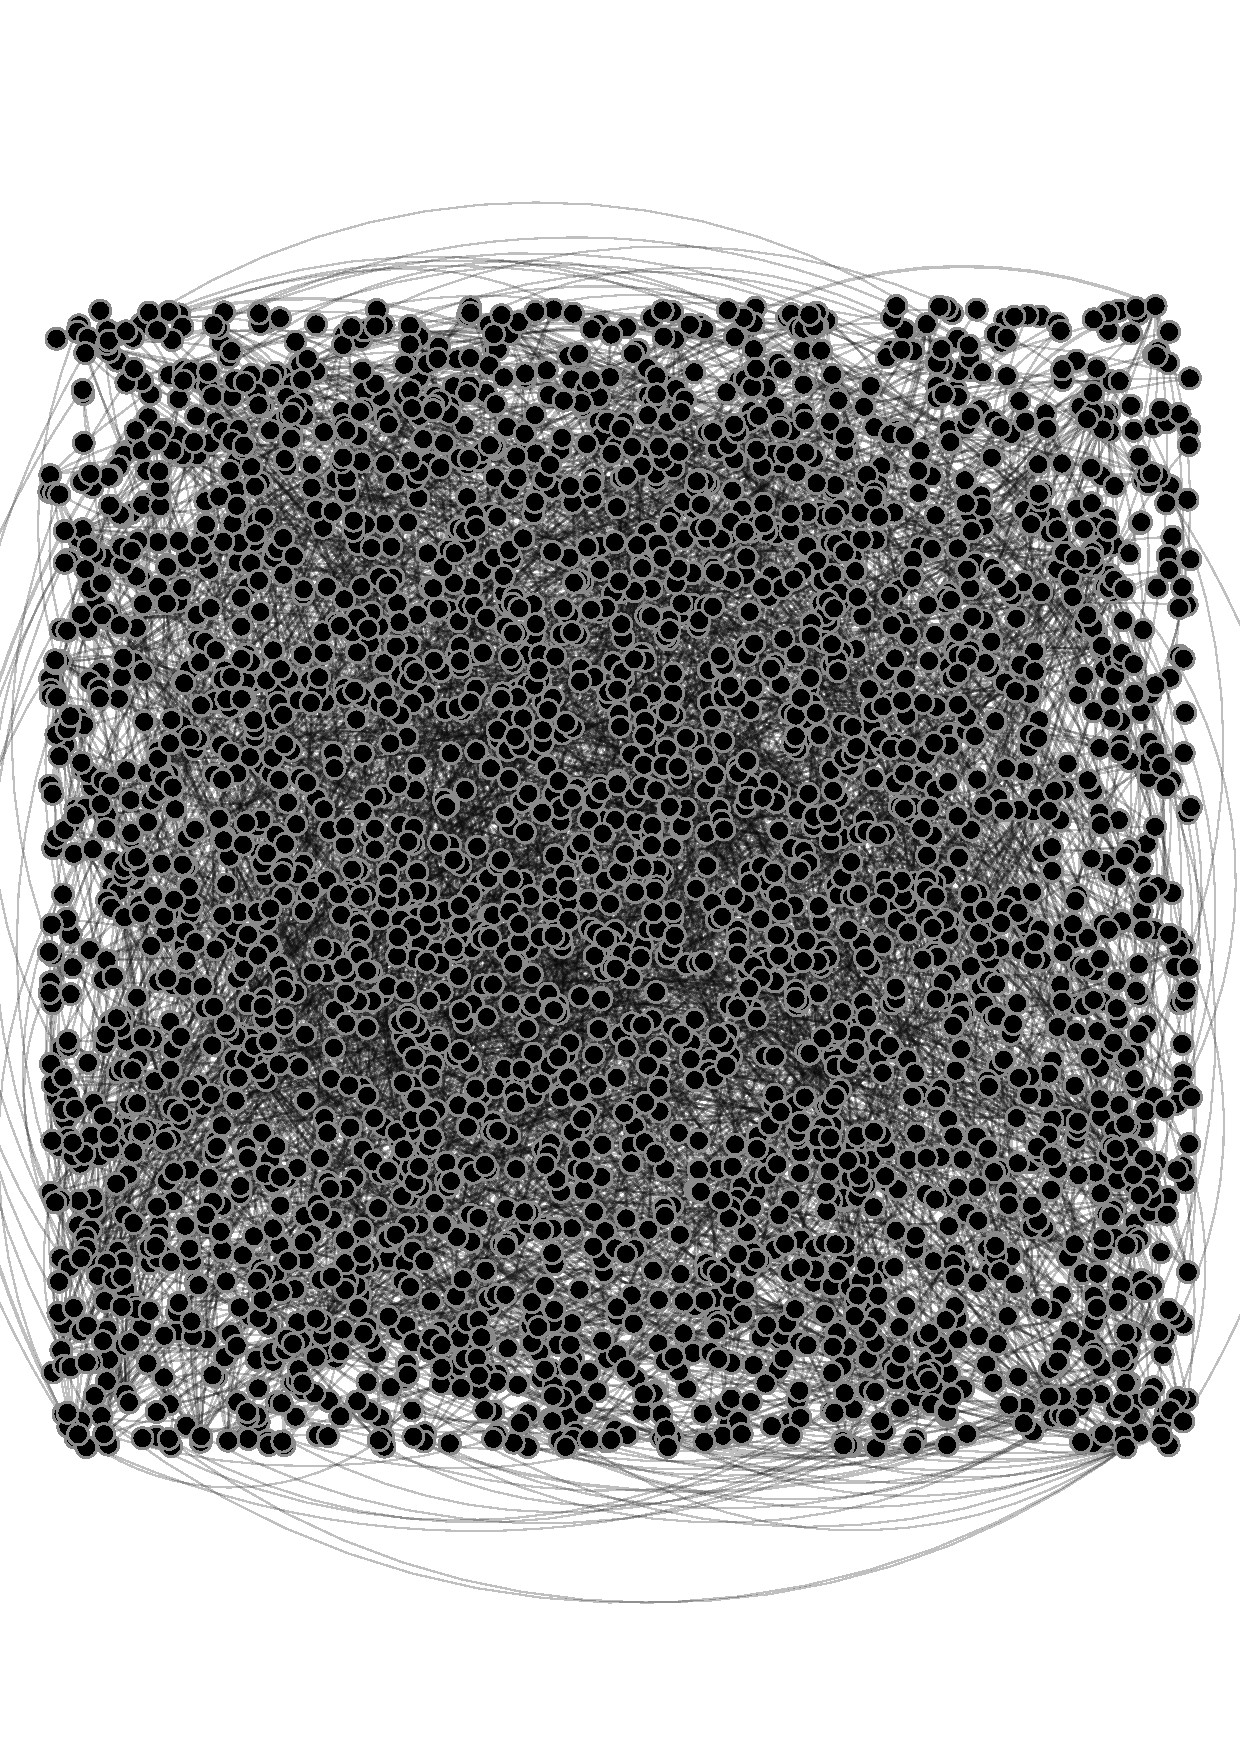
\includegraphics[width=0.55\linewidth]{img/stations}
		\caption{Grafo delle stazioni}
		\label{fig:stationsgraph}
	\end{figure}
	
\subsubsection{Ricerca grafo}
	
		Per la ricerca del percorso più breve tra due stazioni si è utilizzato \textbf{l'algoritmo di Dijkstra}, un algoritmo di ricerca del cammino più breve in un grafo pesato con pesi non negativi, in questo caso specifico il peso di ogni arco è 1, quindi l'algortmo cercherà il percorso con il più piccolo numero di nodi.\\
		\linebreak
		Inizia da un nodo sorgente e calcola le distanze minime da esso a tutti gli altri nodi, mantenendo una coda di priorità, durante l'esecuzione, visita i nodi adiacenti al nodo corrente e aggiorna le distanze minime se trova un cammino più breve. Implementato dalla libreria \textbf{NetworkX}.
		
	\begin{algorithm}
		\caption{Algoritmo di Dijkstra}
		\begin{algorithmic}[1]
			\Procedure{Dijkstra}{$G, s$}
			\State $dist \gets$ array di distanze inizializzato a $\infty$ per tutti i nodi
			\State $dist[s] \gets 0$
			\State $S \gets$ insieme vuoto dei nodi visitati
			\While{$S$ non contiene tutti i nodi}
			\State $u \gets$ nodo non visitato con la minima distanza in $dist$
			\State Aggiungi $u$ a $S$
			\ForAll{nodi adiacenti $v$ di $u$}
			\State $alt \gets dist[u] +$ peso dell'arco tra $u$ e $v$
			\If{$alt < dist[v]$}
			\State $dist[v] \gets alt$
			\EndIf
			\EndFor
			\EndWhile
			\State \textbf{return} $dist$ 
			\EndProcedure
		\end{algorithmic}
	\end{algorithm}

	\textbf{Commento sull'algoritmo} \\
	'''Lorem ipsum dolor sit amet, consectetur adipiscing elit. Maecenas placerat tempus dictum. Vivamus dolor velit, condimentum nec scelerisque nec, blandit at ipsum. Maecenas venenatis sapien vitae rhoncus ultrices. Etiam blandit enim a aliquet sollicitudin. Curabitur ac ligula ac elit dignissim efficitur sed vitae nisi. Aenean porta magna sed pulvinar pretium. Curabitur gravida dolor quis arcu malesuada sodales. Nunc tortor sem, luctus et erat vel, bibendum vestibulum arcu. Integer in tellus mollis, aliquam ipsum vitae, consectetur tortor. Sed vehicula magna ac tristique porttitor. In vel pharetra tellus. Nulla facilisi. '''

	\subsection{Query Knowledge base}
	Per andare ad interagire un Knowledge base vengono eseguite delle \textbf{query}, interrogazioni alla KB, che permettono di estrapolare informazioni specifiche, in questo caso sono state messe a disposizioni delle query predefinite per poter recuperare le informazioni relative ai treni secondo l'esigenze dell'utente. \\
	\linebreak
	In particolare sono state pensate quattro query principali che che verranno eseguite in base alle esigenze dell'utente in base alla ricerca specifica che andrà a fare.\\
	\linebreak
	Query messe a disposizione dal sistema: \\
	
	\textbf{1)} Ricerca di tutti i treni che partono da una determinata stazione
	\begin{figure}[!h]
		\centering
		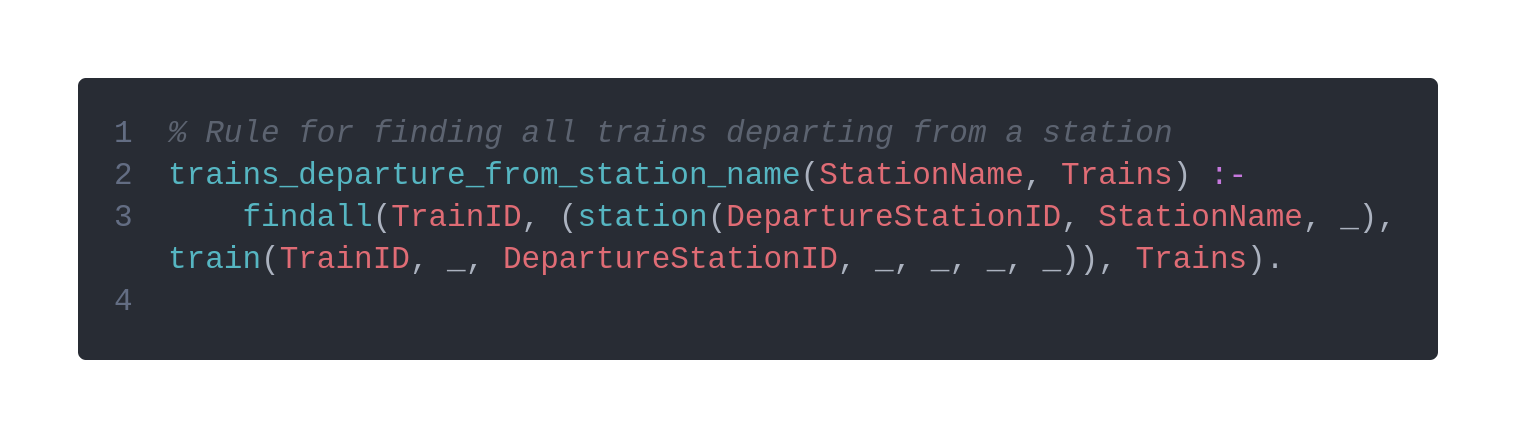
\includegraphics[width=1.1\linewidth]{img/code1}
		\caption{aaaaaaaaaaaaaaaaaaaaaaaaaaaaaaaaaaaaaaaaaaaaaaaaaaaaaaaa}
	\end{figure}

	\textbf{2)} Ricerca di tutti i treni che partono da una determinata stazione da un determinato orario
	\begin{figure}[!h]
		\centering
		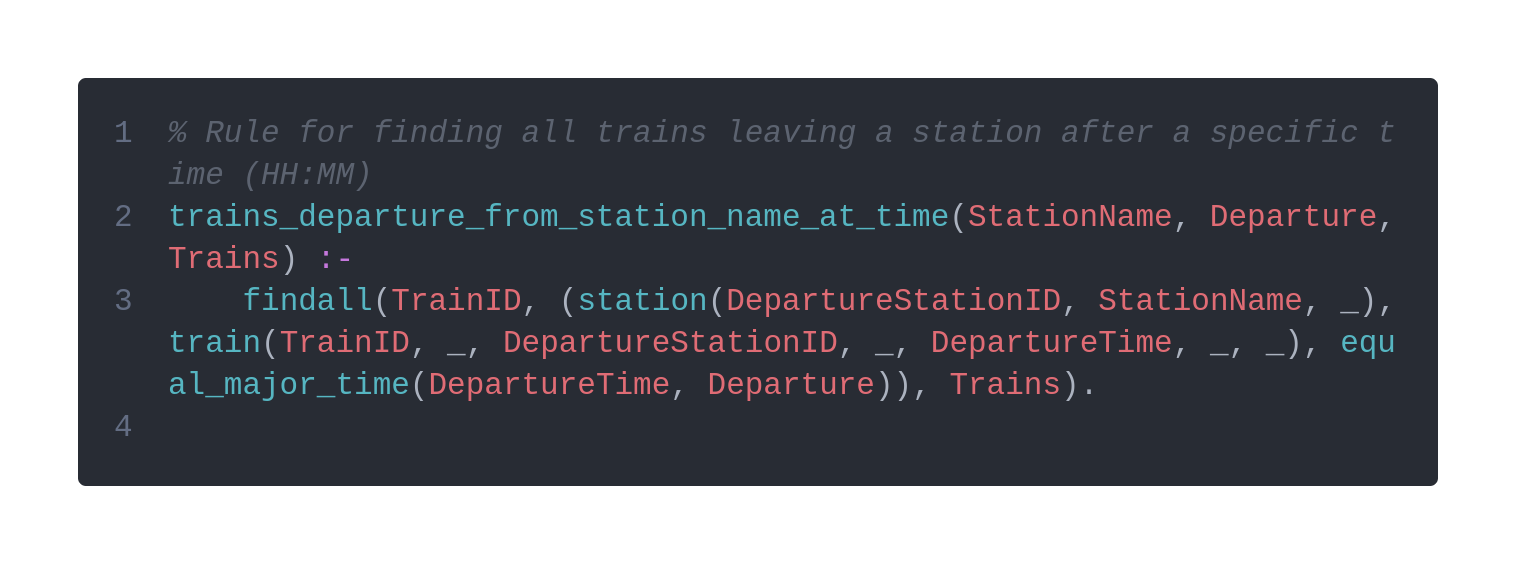
\includegraphics[width=1.1\linewidth]{img/code2}
		\caption{aaaaaaaaaaaaaaaaaaaaaaaaaaaaaaaaaaaaaaaaaaaaaaaaaaaaaaaa}
	\end{figure}

	\textbf{4)} Ricerca di tutti i treni disponibili tra due stazioni
	\begin{figure}[!h]
		\centering
		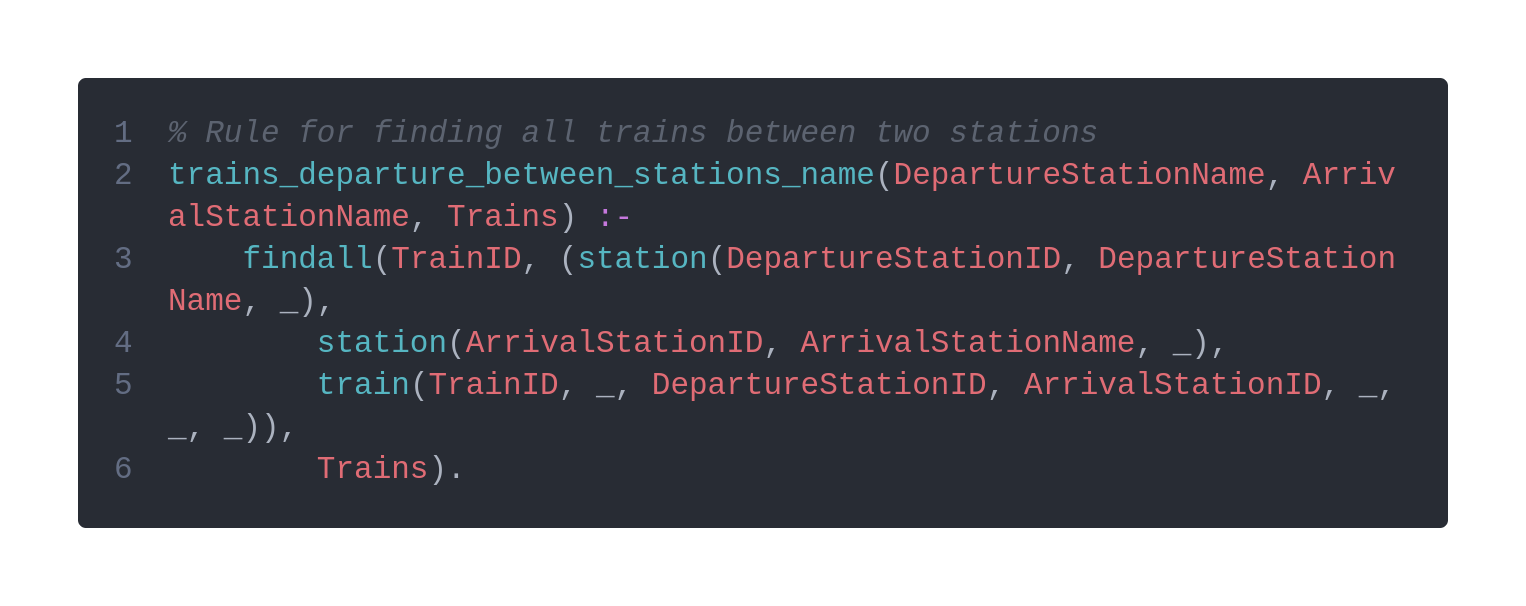
\includegraphics[width=1.1\linewidth]{img/code3}
		\caption{aaaaaaaaaaaaaaaaaaaaaaaaaaaaaaaaaaaaaaaaaaaaaaaaaaaaaaaa}
	\end{figure}	
	
	\textbf{3)} Ricerca di tutti i treni disponibili tra due stazioni dopo un determinato orario
	\begin{figure}[!h]
		\centering
		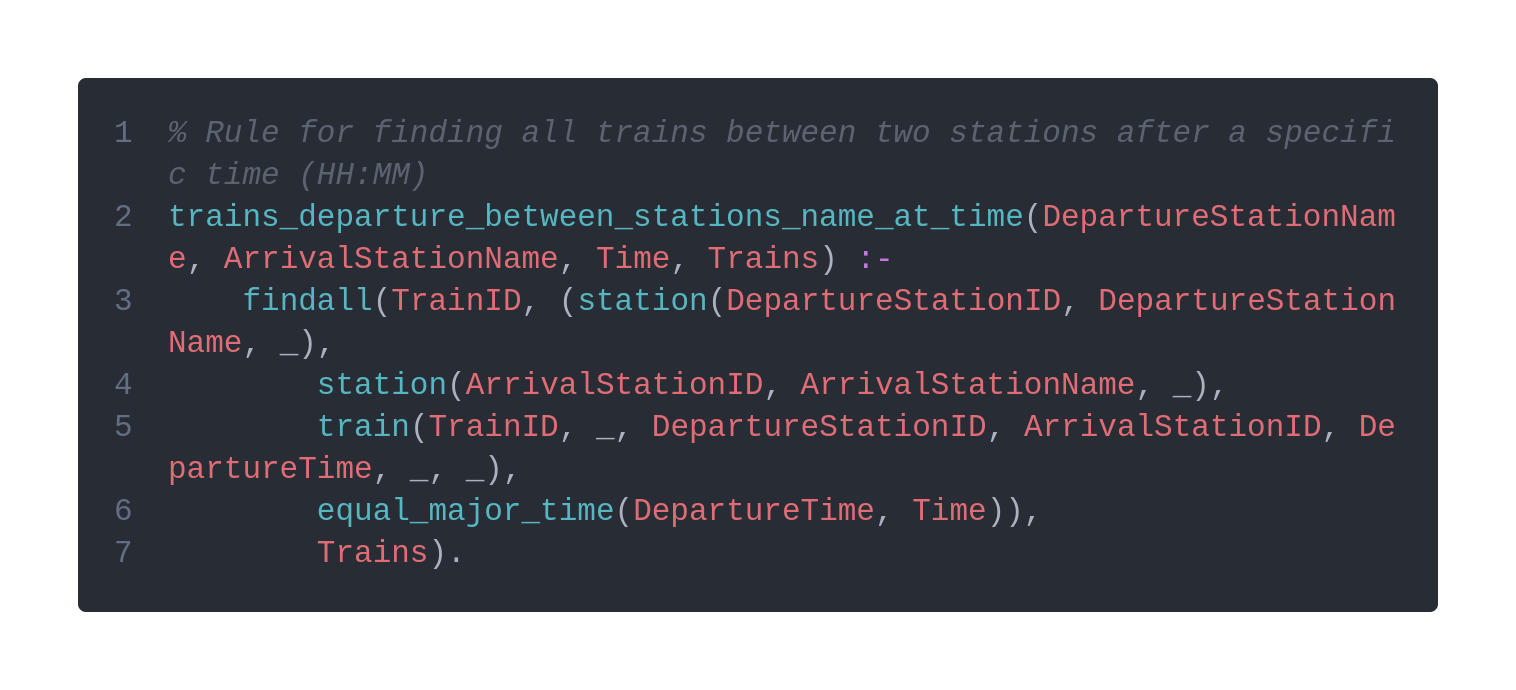
\includegraphics[width=1.1\linewidth]{img/code4}
		\caption{aaaaaaaaaaaaaaaaaaaaaaaaaaaaaaaaaaaaaaaaaaaaaaaaaaaaaaaa}
	\end{figure}
\linebreak
	Oltre queste query sono state prodotte altre regole, di supporto, per il funzionamento interno di queste principali, come quella per convertire le stringhe che rappresentano gli orari dal formato \textit{"HH:MM"} in minuti, quella per reperire tutte le info dei treni dall'id, etc\dots

	\section{Machine Learning}
	
	\subsection{Origine dataset}
		Il dataset di addestramento e test è stato recuperato per mezzo dell'interrogazione tramite API al serivio 	\href{http://www.viaggiatreno.it/infomobilita/index.jsp}{viaggiotreno.it}, in particolare si sono recuperate le informazoni giornaliere circa i treni (ID, tipo di treno, ...) ed in più il ritardo effettuato della corsa specifica.
		
	\subsection{Analisi del dataset}
		Il dataset ottenuto è composto da 101169 osservazioni per otto features che, come già detto sopra, vanno a descrivere una serie di caratteristiche legate all'andamento giornaliero dei treni, abbiamo:
		
		\begin{enumerate}
			\item \textit{train\_id}[numeric]: identificatore univoco del treno,
			\item \textit{origin}[string]: nome della stazione di partenza,
			\item \textit{arrival}[string]: nome della stazione di arrivo,
			\item \textit{departure\_time}[string]: orario di partenza (HH:MM),
			\item \textit{arrival\_time}[string]: orario di arrivo (HH:MM),
			\item \textit{delay}[numeric]: ritardo registrato,
			\item \textit{train\_type}[string]: tipo di treno, regionale o nazionale,
			\item \textit{detection\_date}[date]: data della corsa.
		\end{enumerate}
		Ecco un esempio:
		
			\begin{figure}[!h]
				\centering
				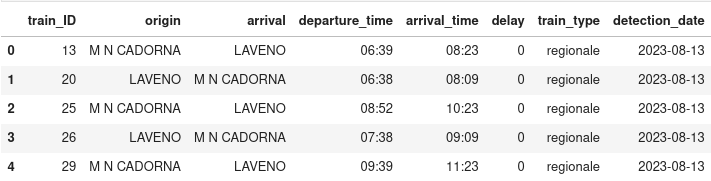
\includegraphics[width=1.1\linewidth]{img/dataset}
				\caption{aaaaaaaaaaaaaaaaaaaaaaaaaaaaaaaaaaaaaaaaaaaaaaaaaaaaaaaa}
			\end{figure}
	

	\subsection{Preparazione dati}
		Prendedo il dataset così descritto ci sono una serie di problematiche da risolvere per poter usare i dati, in particolare andando a considerare le osservazioni notiamo che per i valori nominali, in questo caso quelli che esprimono il nome della stazione di partenza e di arrivo, ci sono dei caratteri che andrebbero modificati per formattare meglio il dataset, in particolare si sono andati a sostituire i punti, le virgole, gli accenti e le doppie virgolette con degli underscore per poter meglio gestire il dataset.
		
		\subsubsection{Analisi input features}
			Considerando le feature di input, cioè quelle sulle quali il modello andrà ad imparare, non tutte sono importanti per per il raggiongimento del nostro scopo, in particolare si sono escluse:
			
			\begin{itemize}
				\item \textit{origin} (il modello scelto non accetta dati di tipo string),
				\item \textit{arrival} (il modello scelto non accetta dati di tipo string),
				\item \textit{detection\_date} (nessuna correlazione sulle feature su cui fare predizione).
			\end{itemize}
			Per quanto riguarda le feature rimanenti si è optato per una trasformazionde dei valori per adattarli al modello, specificatamente i valori di \textit{departure\_time} e \textit{arrival\_time} da stringhe nel formato HH:MM si è passati a valori numerici che rappresentano i minuti ($hour*60+minutes$), inoltre si è operato anche su \textit{train\_type} eseguendo una binarizzazione:
			\begin{equation*}
				\begin{cases}
					1 \quad \text{per } train\_type(i) = regionale \\
					0 \quad \text{per } train\_type(i) = nazionale
				\end{cases}
			\end{equation*}
			
		\subsubsection{Analisi target feature}
			La target feature rappresenta l'biettivo sella notra predizione, in questo caso \textit{delay} che rappresenta il ritardo di una detrminata corsa, essendo un task di classificazione, cioè prevedere se un determinato treno farà ritardo o meno, anche in questo caso si è eseguita una binarizzazione:
			
			\begin{equation*}
				\begin{cases}
					1 \quad \text{per } delay(i) > 0  \\
					0 \quad \text{otherwise}
				\end{cases}
			\end{equation*}
			\linebreak
			\\
			Nel dataset abbiamo una distribuzione abbastanza bilanciata dei valori per la feature \textit{delay}
			
			\begin{figure}[!h]
				\centering
				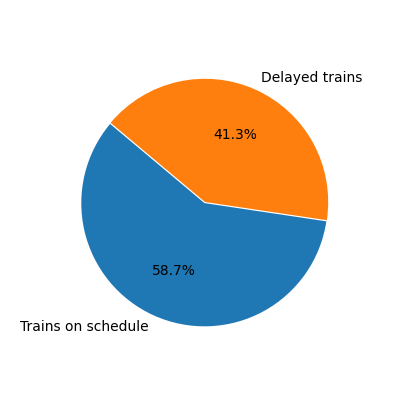
\includegraphics[width=270px]{img/delay_graph}
				\caption{Distribuzione dei treni con e senza ritardo}
			\end{figure}
			
	\subsection{Apprendimento automatico}
	Per produrre un modello che va predire se un treno farà ritardo o meno di ricorre all'apprendimento automatico o \textit{machine learning} che consiste nell'addestrare i computer a imparare dai dati e a migliorare le proprie prestazioni nei compiti specifici senza essere esplicitamente programmanti.\\
	\linebreak
	Per questo caso speficico si è usata la \textbf{Random forest}, modello di apprendimento automatico che combina molteplici alberi decisionali (decision trees), ulteriore modello, per migliorare la previsione e la generalizzazione.\\
	La random forest fa parte della gamma dei modelli di \textbf{apprendimento supervisionato}, cioè viene addestrato su un insieme di dati di addestramento che includono sia le caratteristiche (input features) che le risposte corrette (output features). 
	Il modello impara a fare previsioni basate su questi esempi etichettati. \\
	\linebreak
	In particolare la Random Forest funziona creando un insieme di alberi decisionali, ognuno addestrato su un subset casuale dei dati di addestramento e su un subset casuale delle caratteristiche.\\
	Questo processo introduce variabilità e riduce il rischio di sovradattamento (overfitting). Quando si effettua una previsione, ciascun albero fornisce una previsione, e la Random Forest combina queste previsioni per ottenere un risultato finale più accurato e stabile. 
	
	\begin{figure}[!h]
		\centering
		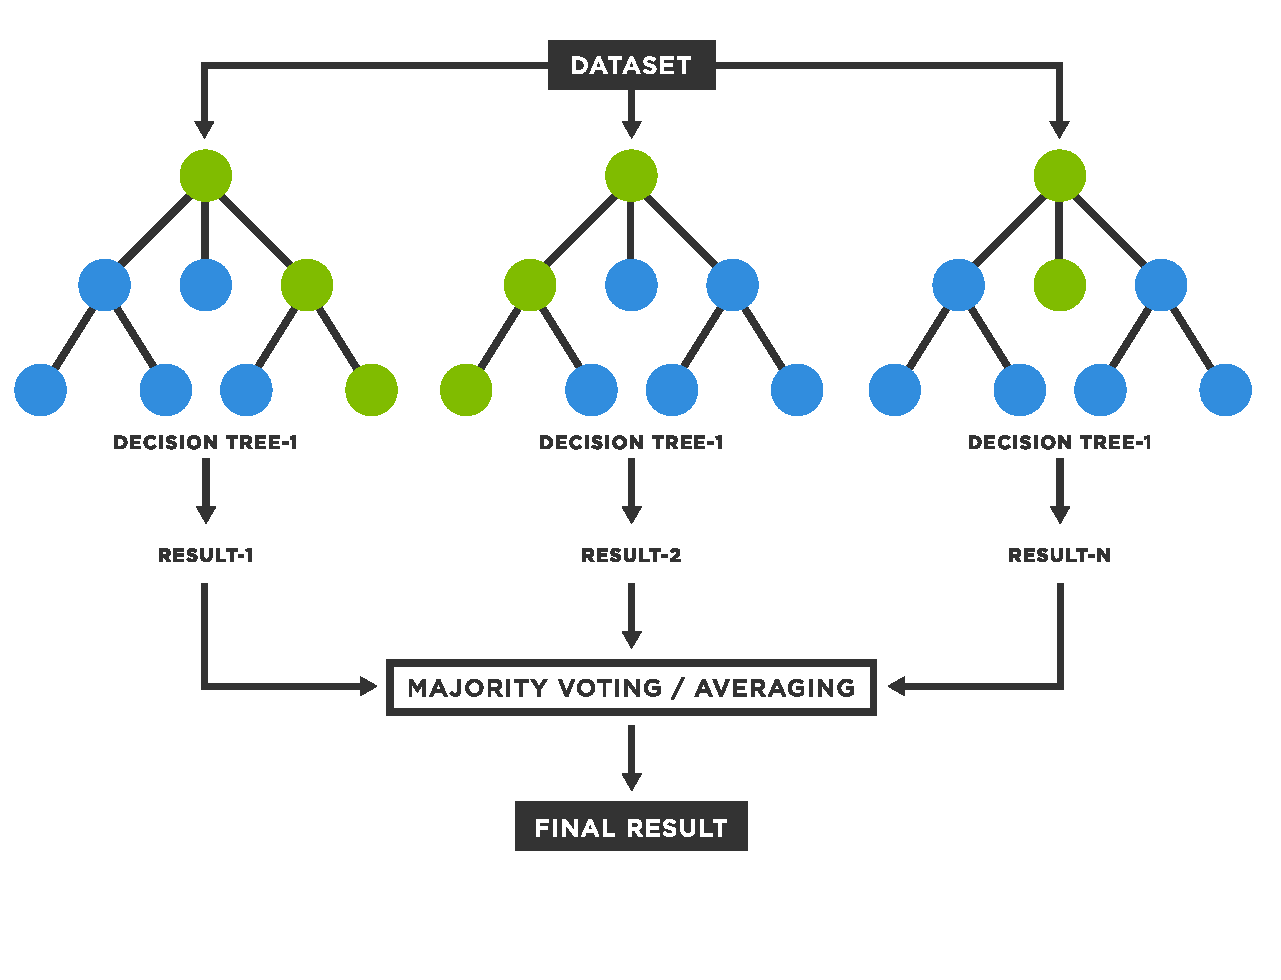
\includegraphics[width=270px]{img/random-forest-diagram}
		\caption{Esempio di random forest}
	\end{figure}
	

		\footnote{Fonte: \href{https://www.spotfire.com/glossary/what-is-a-random-forest}{www.spotfire.com}}

	
	
	\subsection{Valutazione dei modelli}

	
	\subsubsection{Metriche scelte}


	\section{Risultati}


	
	\subsubsection{Considerazioni}
	
	\section{Sviluppi futuri}
	Il sistema presentato è aperto a sviluppi futuri che possano rendere il sistema ancora più efficiente e all'avanguardia. \\
	Di seguito sono descritti alcuni dei possibili sviluppi futuri che intendiamo esplorare:
	
	\begin{enumerate}
		\item Espansione della copertura ferroviaria andando a completare le informazioni relative a treni e staziono ed integrazione con altri servizi ferroviari (Italo, Frecciarossa, ...)
		\item Implementazione di una vera e propria interfaccia grafica
		\item Miglioramento della ricerca andando a suggerire all'utente, sulla base dei caratteri inseriti, le stazioni che iniziano con quei caratteri
		\item Integrazione di dati in tempo reale andando a fornire all'utente informazioni in \textit{real time}

	\end{enumerate}
	\printbibliography
	
\end{document}